	\documentclass[10pt,a4paper]{report}
	\usepackage{graphicx}
	\usepackage[utf8]{inputenc}
	\usepackage{amssymb,amsmath}
	\usepackage{geometry}

\usepackage[colorlinks = true,
            linkcolor = blue,
            urlcolor  = blue,
            citecolor = blue,
            anchorcolor = blue]{hyperref}

	\usepackage{bookmark}
    \usepackage{wrapfig}
	%\geometry{article}
    \usepackage[final]{pdfpages}
	\usepackage[ampersand]{easylist}	
    \newcommand\tab[1][1cm]{\hspace*{#1}}

\hypersetup{
	pdftitle={Digital integrated circuit design},%
	pdfauthor={Matteo Baldo},%
	pdfsubject={Digital integrated circuit design},%
	pdfkeywords={},%
	colorlinks=true,%
	linkcolor=blue,%
	linktocpage=true,%
	pageanchor=true
}


\begin{document}

% INIZIO PRIMA PAGINA DI INTRODUZIONE
\begin{titlepage}

	\centering
	{\scshape\huge\textbf Digital integrated circuit design \par}
	{\scshape\huge\textbf Notes \par}	
	\vspace{13cm}
{Professor:\\ \textit{Andrea Bonfanti}}	

\vspace{0.5cm}

{Student:\\ \textit{Matteo Baldo}}

\vspace{2cm}
	\vfill
	\raggedleft
	{\today\par}
	
\vspace{1cm}
\raggedright
{ \it ...and so on and so forth ...}
\end{titlepage}
% FINE PRIMA PAGINA DI INTRODUZIONE
        \newpage
		\setcounter{page}{2}
        \null 
        \thispagestyle{empty} 
        \newpage  


\pdfbookmark{\contentsname}{Index}
\tableofcontents
        % Intro page and index
%------------------------------------------------------------------------%
\newpage 


\begin{center}
\vspace*{\stretch{1}}
If you want to find the source code of this pdf or more material of other topics please visit my github account\\
\url{https://github.com/matteobaldo}
\vspace*{\stretch{1}}
\end{center}
            % Reference on github page 
%------------------------------------------------------------------------%
\chapter{The MOS transistor}
\section{Symbols}
The symbols used to draw n and p MOS transistors in digital electronics are the one show in figure below

\centering
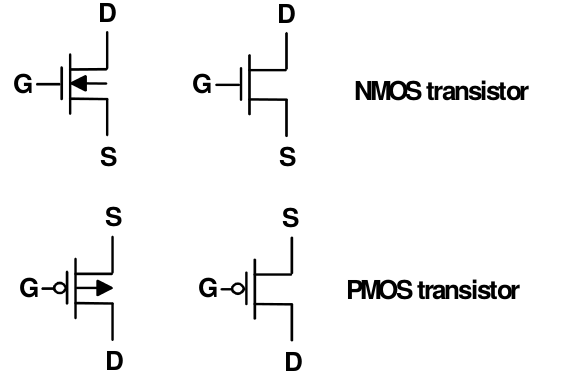
\includegraphics[width=0.35\textwidth]{C2_1.png}\\
\raggedright



\section{Working regimes}
We are intrested in the use of MOS transistors as swithces and not as amplifiers.\\
In our analysis we will consider the following operating regions with the corrisponding voltages 

\centering
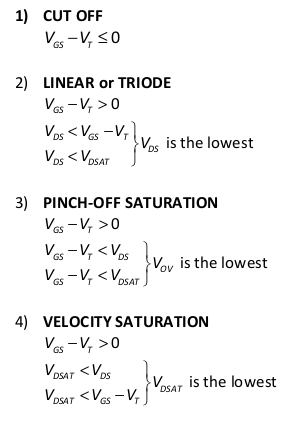
\includegraphics[width=0.3\textwidth]{C2_2.png}\\
\raggedright

and to assest the right expression of the current we will use the following unified model 


\centering
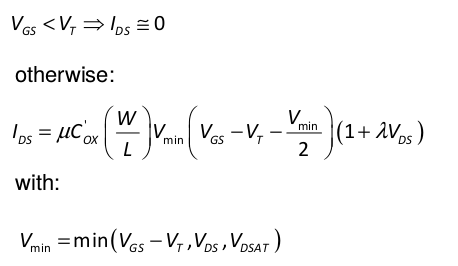
\includegraphics[width=0.5\textwidth]{C2_3.png}\\
\raggedright

In the reference technology of this course (bulk CMOS 0.25$\mu m$) this are the characteristics parameters

\centering
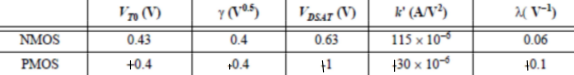
\includegraphics[width=0.7\textwidth]{C2_4.png}\\
\raggedright

\subsection{Body effect}

Since the $V_t$ depends on the source-body potential if this value is different form 0 we get

\centering
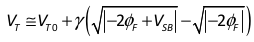
\includegraphics[width=0.35\textwidth]{C2_5.png}\\
\raggedright

where $\gamma$ is the body effect coefficient.

\subsection{Subthreshold regime}

When the overdrive voltage is equal to 0 the current in the device is not exactly 0 but the device enters in the so called subthreshold regime where the current behaves like in an BJT junction 

\centering
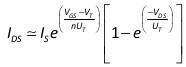
\includegraphics[width=0.35\textwidth]{C2_6.png}\\
\raggedright

this current is crucial in the power consumption in off mode.\\

\section{Equivalent resistance}
We can define an equivalent resistance of the MOS transistor as

\centering
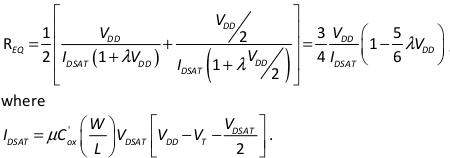
\includegraphics[width=0.5\textwidth]{C2_7.png}\\
\raggedright

the last term in parentesis can be easily neglected since is $\simeq 1$.\\
We can make three considerations:\\
\tab 1)the resistance is inversely proportional to the (W/L) ratio of the device\\
\tab 2)for $V_{DD} >> V_T + V_{DSAT}/2$, the resistance becomes virtually independent of the supply voltage\\
\tab 3)once the supply voltage approaches $V_{TE} =0.745V=V_T+V_{DSAT}/2$, a dramatic increase in resistance can be observed,even if the model adopted (considering the velocity saturation) is no longer valid\\
\vspace{5mm}
In digital electronics once we have the equivalent resistance of the MOS, we can evaluate the propagation time on the basis of the RC model, as $\ln(2)RC$.\\














        %The MOS transistor
%------------------------------------------------------------------------%
\chapter{The CMOS inverter}

\centering
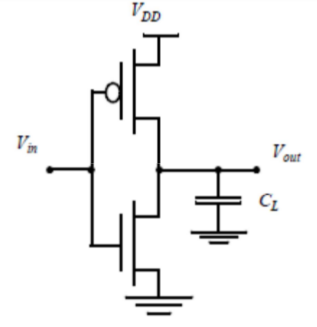
\includegraphics[width=0.35\textwidth]{C3_1.png}\\
\raggedright

We will refer to CMOS inverter implemented in a static FC-CMOS logic. FC-COMS means fully-complementary logic, which is a particular class of static gates.
Static refers to the fact that these gates have an output node always connected to GND or VDD through a low impedance path. Fully-complementary means that the gate is composed by a pull-down network and a complementary pull-up network.\\

\section{Static behavior}

Independently of the transistor size the high and low output levels are equal to $V_{DD}$ and GND that in out reference technology are 2.5V and 0V
\begin{equation}
V_{OH}=V_{DD}=2.5V
\end{equation}
\begin{equation}
V_{OL}=GND=0V
\end{equation}
This two values are indipentent form the relative device size; gates with this propriety are called ratioless (gates without this propriety are ratioead).\\
\vspace{5mm}
There is always in steady state a finite resistance between the output node and GDN or VDD (that isn't the equivalent resitance of the previous chapter that is useful to assest the propagation delay).\\
For VDD=2.5V we get
\begin{equation}
r_{on}=\frac{4.2k}{(W/L)_n}\ \ \ \ \ \ \ \ \ \ r_{on}=\frac{15.9k}{(W/L)_p} 
\end{equation}

\centering
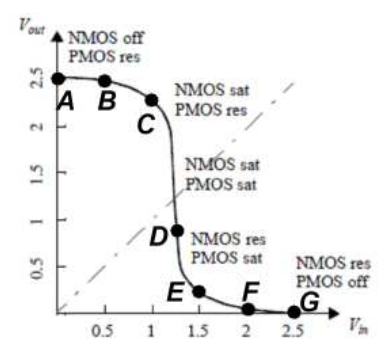
\includegraphics[width=0.35\textwidth]{C3_2.png}\\
\raggedright



\subsection{Switching threshold}
Let's suppose that during the transistion both transistor are in velocity saturation region (this is not correct but leads to a negligible error) to assest the threshold voltage $V_M$ of the inverter we have to put the 2 currents of the mos equal doing this we obtain 

\vspace{2.5mm}

\centering
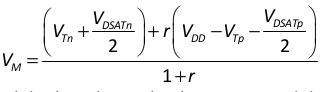
\includegraphics[width=0.35\textwidth]{C3_3.png}\\
\raggedright
 
with 

\centering
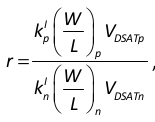
\includegraphics[width=0.15\textwidth]{C3_4.png}\\
\raggedright

We can oslo have the following inverse relationship

\vspace{2.5mm}

\centering
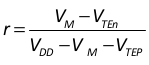
\includegraphics[width=0.15\textwidth]{C3_5.png}\\
\raggedright

For $V_M=1.25V$ that is the best case we get
\begin{equation}
\frac{(W/L)_p}{(W/L)_n}=3.5\simeq 3
\end{equation}

\subsection{Noise marigns}

To compute $V_{IL}$, $V_{IH}$ we consider the piecewise linear approximation for the VTC, where the transition region is approximated by a straight line having the same negative slope of original VTC in the threshold point.\\

\centering
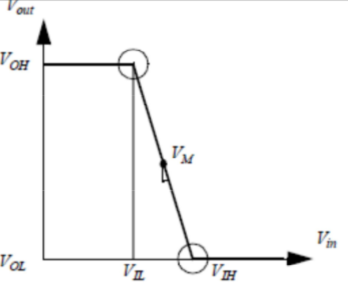
\includegraphics[width=0.35\textwidth]{C3_6.png}\\
\raggedright

In this way the straight line that approximates the VTC near the threshold is 
\begin{equation}
V_{OUT}=V_{IN}g+(1-g)V_M \ \ \ \ \ \ (g<0)
\end{equation}
we can compute g considering that $g=-(g_{mn}+g_{mp})r_{0p}//r_{0p}$ we obtain

\vspace{2.5mm}

\centering
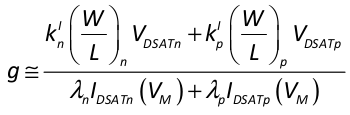
\includegraphics[width=0.35\textwidth]{C3_7.png}\\
\raggedright

\vspace{2.5mm}

The gain is apporoximately constant if the velocity saturation is taken into account.\\

From this we get 

\centering
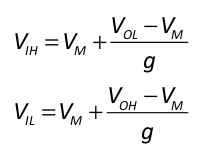
\includegraphics[width=0.15\textwidth]{C3_8.png}\\
\raggedright

\centering
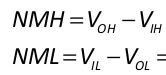
\includegraphics[width=0.11\textwidth]{C3_9.png}\\
\raggedright

\section{Dinamic behavior}


\centering
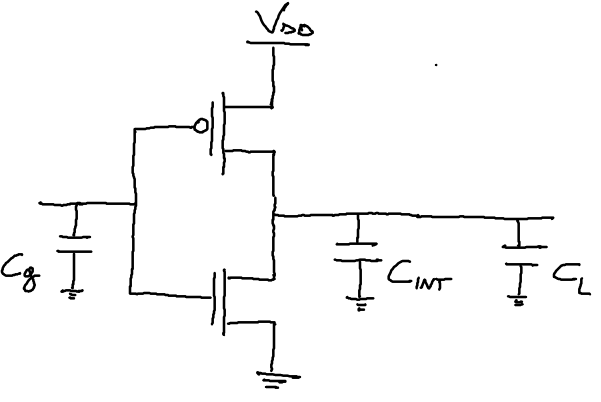
\includegraphics[width=0.45\textwidth]{C3_10.png}\\
\raggedright

We define the following parameters \\
\tab $W_n,W_p$ the width of the drain junctions (that is the same of W/L)\\
\tab $L_D$ Drain length (that isn't the same as W/L)\\
\tab $A_{d}=W*L_D$ the area of the drain\\
\tab $P_{d}=2L_D+W$ the perimeter of the drain\\


\subsection{Intinsic capacitance $C_{int}$}
\vspace{2mm}
\begin{equation}
C_{int}=C_{overlap}+C_{dbn}+C_{dbSWn}+C_{dbp}C_{dbSWp}
\end{equation}
{\bf Overlap capacitance}\\
\begin{equation}
C_{ovelap}=2(C'_{ovp}W_p+C'_{ovn}W_n)
\end{equation}
\vspace{5mm}
{\bf Drain-bulk n capacitances}
\begin{equation}
C_{dbn}=\frac{C'_{jn}A_{dn}}{2}\left(\frac{1}{(1+\frac{V_{DD}}{\phi})^{0.5}}+\frac{1}{(1+\frac{V_{DD}}{2\phi})^{0.5}}  \right)
\end{equation}

\begin{equation}
C_{dbSWn}=\frac{C'_{jSWn}P_{dn}}{2}\left(\frac{1}{(1+\frac{V_{DD}}{\phi})^{0.44}}+\frac{1}{(1+\frac{V_{DD}}{2\phi})^{0.44}}  \right)
\end{equation}

\vspace{5mm}
{\bf Drain-bulk p capacitances}
\begin{equation}
C_{dbp}=\frac{C'_{jp}A_{dp}}{2}\left(1+\frac{1}{(1+\frac{V_{DD}}{2\phi})^{0.48}}  \right)
\end{equation}

\begin{equation}
C_{dbp}=\frac{C'_{jSWp}P_{dp}}{2}\left(1+\frac{1}{(1+\frac{V_{DD}}{2\phi})^{0.32}}  \right)
\end{equation}


\subsection{Gate capacitance $C_{g}$}

\begin{equation}
C_g=C'_{ovn}W_n+C'_{ovp}W_p+C'_{ox}(W_nL_n+W_pL_p)
\end{equation}

\subsection{Self-loading factor}
We can define the self-loading factor $\gamma$ as 
\begin{equation}
C_{int}=\gamma C_g
\end{equation}
In our reference technology we have $\gamma=1$ and $C_g^{(1)}=2fF$ where the suffix (1) is the size of the inverter (that is the W/L of the n-mos).\\
If we have an inverter of size $\alpha$ it's gate capacitance will be 
\begin{equation}
C_g^{(\alpha)}=\alpha C_g^{(1)}=\alpha\cdot 2fF
\end{equation}


\section{Propagation delay}
\centering
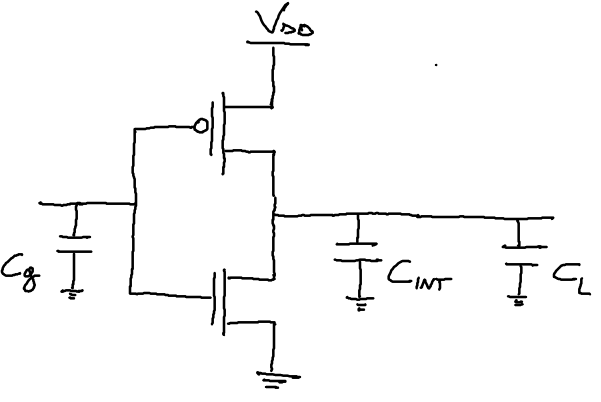
\includegraphics[width=0.45\textwidth]{C3_10.png}\\
\raggedright

Propagation delay form high to low

\centering
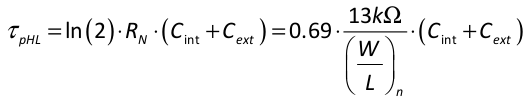
\includegraphics[width=0.35\textwidth]{C3_11.png}\\
\raggedright

\vspace{5mm}

Propagation delay forom low to high 

\centering
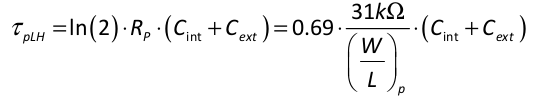
\includegraphics[width=0.35\textwidth]{C3_12.png}\\
\raggedright

\vspace{5mm}
We define intrinsic propagation delay as the average between this 2 results when $C_{ext}=0$
\begin{equation}
\tau_{p0}=\frac{\tau_{HL}+\tau_{LH}}{2}
\end{equation}

\subsection{Fan-out}
Considering an external capacitance we get the folowing expression
\begin{equation}
\tau_p=\ln(2)R_{eq}(C_{int}+C_{ext})=\tau_{p0}\left(1+\frac{C_{ext}}{C_{int}}\right)=\tau_{p0}\left(1+\frac{C_{ext}}{\gamma C_g}\right)=\tau_{p0}\left(1+\frac{f}{\gamma}\right)
\end{equation}
Where we used the fan-out f and the self-loading factor defined as
\begin{equation}
f=\frac{C_{ext}}{C_g}\ \ \ \ \ \ \ \ \ \ \ \ C_{int}=\gamma C_g
\end{equation}

\section{Chain of inverters}

To optimize the propagation delay of an inverter chain with N elements we have to set all propagation delay of the inverters equal $f_i=f_i+1\ \ \  \forall i=0,...,N$.\\
To do this we have to calculate the path fan-out that is the load over the first gate capcitance
\begin{equation}
F=\frac{C_L}{C_{g,1}}
\end{equation} 
And from this we calculate the optimum fan-out 
\begin{equation}
f_{opt}=\sqrt[N]{F}
\end{equation}
given the first inverter size $s_1$ all the other inverters' dimensions are fixed 
\begin{equation}
s_n=s_1\cdot (f_{opt})^{n} \ \ \ \forall n=1,...,N 
\end{equation} 
and the propagation delay is 
\begin{equation}
\tau_p=N\tau_{p0}\left(1+\frac{f_{opt}}{\gamma} \right)
\end{equation}

\vspace{5mm}

If the number of inverter isn't fixed we can compute for our reference technology the optimum number of stages as 
\begin{equation}
N_{opt}=\frac{\ln(F)}{\ln(3.6)}
\end{equation}
beacuse the best fan-out that we can have is 
\begin{equation}
f_{opt}^{ideal}=3.6
\end{equation}
Of course the number of stages N has to ben an integer number.\\

        %The CMOS inverter
%------------------------------------------------------------------------%
\chapter{Inverter power consumption}

\section{Dynamic power consumtion}
Only in case of charge of a capacitance so in a LOW to HIGH transition at the output of an inverter. \\
The most general formula for the power dissipated in this process is
\begin{equation}
P_{dyn}=C_LV_{DD}^2f_{1\rightarrow 0}
\end{equation}
where $f_{1\rightarrow 0}$ is the frequency of the 0-1 transition at the output node. This term can be deconposed in 2 factor the clock of the circuit and the switching activity $\alpha_{SW}$ that is the probability to have a transition from 0 to 1 at the output.\\
\vspace{2mm}
\tab In case of a square wave we have 
\begin{equation}
f_{1\rightarrow 0}=f_{clk}\cdot \alpha_{SW}=f_{clk}\cdot \frac{1}{2}
\end{equation}
\tab In case of a randoom signal 
\begin{equation}
f_{1\rightarrow 0}=f_{clk}\cdot \alpha_{SW}=f_{clk}\cdot \frac{1}{4}
\end{equation}
\vspace{5mm}
In the end we can write this 2 final equation for dynamic power dissipation
\begin{equation}
P_{dyn}=C_LV_{DD}^2 f_{clk}\cdot \alpha_{SW}
\end{equation}
\begin{equation}
E_{dyn}=C_LV_{DD}^2\alpha_{SW}
\end{equation}
In case of a chain of inverters $C_L$ is the sum of all the capacitance at the output nodes of the single inverters.\\

\section{Cross-conduction power consumption}
Due to the finite slope of the input signal there is a finite time when both p-mos and -mos are on creating a low impedance path between $V_{DD}$ and GND.\\

\centering
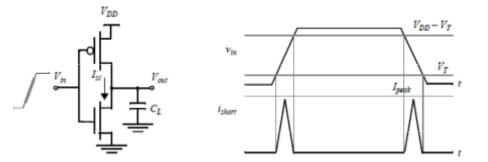
\includegraphics[width=0.7\textwidth]{C4_1.png}\\
\raggedright

\centering
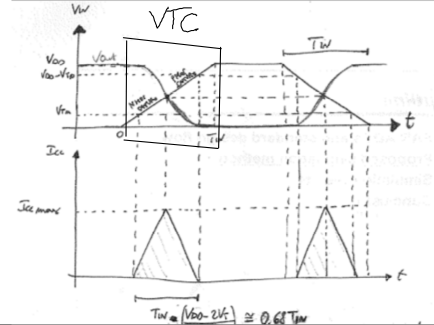
\includegraphics[width=0.5\textwidth]{C4_1b.png}\\
\raggedright

Defining $T_{in}$ as the time needed by the input signal to transition from GND to $V_{DD}$ and vice-versa and $I_{peak}$ the velocity saturation current of the n-mos (when the input and the output are at $V_m$) we can compute the cross-conduction energy as (assuming $V_{tp}=V_{tn}$) 
\begin{equation}
E_{cc}= \frac{1}{2} V_{DD}I_{peak}\cdot 0.68 \cdot T_{in}
\end{equation}
If we consider an input signal with an update frequency of f with continuos switch HL LH the power is 
\begin{equation}
P_{cc}=\frac{V_{DD}I_{peak} \cdot 0.68 \cdot T_{in}}{2} f
\end{equation}

\vspace{5mm}

With capacitve loads the cross-conduction power becomes smaller than without.\\ 
The cross conduction power can be neglected when 
\begin{equation}
T_{in}<10\tau_p
\end{equation}
with $\tau_p$ propagation delay of the stage.\\


\section{Static power consumption}
It's due to the subthreshold current of the MOS devices.

        %Inverter power consumption
%------------------------------------------------------------------------%
\chapter{The wires}

To simplify the analysis of the wires parasitics effects we introduce 3 simple assumption;\\
\vspace{2mm}
\tab $\rightarrow$ Inductance can be neglected if the wire resistance is large or if the rise/fall time of the input signal is large.\\
\vspace{2mm}
\tab $\rightarrow$ When the wire is short and when the equivalent resistance of the driver is large, the wire resistance can be serenely neglected.\\
\vspace{2mm}
\tab $\rightarrow$ When the separation between nearby wires is large or when the wires run in parallel for a short distance, the inter-wires capacitance can be neglected.\\


%------------------------------------------------------------------------%
%------------------------------------------------------------------------%
\section{Capacitance}

\centering
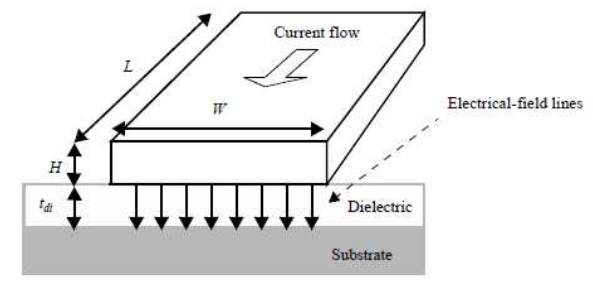
\includegraphics[width=0.5\textwidth]{C5_1.png}\\
\raggedright

We divide the overall capacitance of a wire in 2 main contribution; parallel plate capacitance and fringing capacitance.\\
In the ideal case where the parameter $W/t_{di}$ is very large the fringing capacitance contribution can be neglected but since in our reference technology we can have $W/H>1$ the fringing or border capacitance is the dominant contribution.\\
\vspace{5mm}

For our reference technology process the following table is given reporting the parallel-plate and the fringing capacitance contributions for a wire in a certain layer with respect to another wire in another layer.\\
The parallel-plate capacitance is reported in the white rows expressed in $aF/\mu m^2$ of overlapping area, while the shaded rows report the fringing capacitance contribution in $aF/\mu m$ of perimeter (that is quite always $\simeq 2L$).\\

\centering
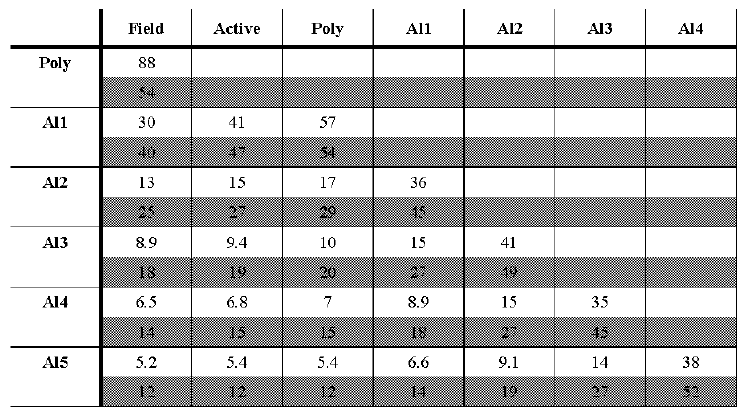
\includegraphics[width=0.8  \textwidth]{C5_2.png}\\
\raggedright
When using this table we have always to look what tipe of metal is our wire (rows) and in what material is made the ground plane or the other wire (columns) in order to get the correct values.\\

\vspace{3mm}
To evaluate che capacitance of 2 nearby wires implemented in the same layer at minimum distance we get the following table with the vales of the capacitances for unit lenght expressed in $aF/\mu m$ \\
\vspace{3mm}

\centering
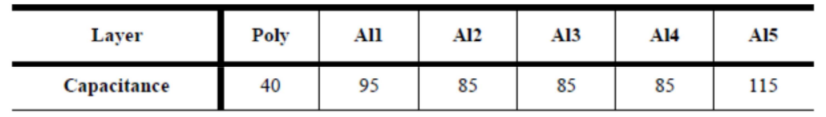
\includegraphics[width=0.8\textwidth]{C5_3.png}\\
\raggedright


%------------------------------------------------------------------------%
%------------------------------------------------------------------------%
\section{Resistance}

Resistance of a wire can be assested as
\begin{equation}
R=\rho \frac{L}{WH}=R_{sh}\frac{L}{W}
\end{equation} 
where the last part represent the resistance per square multiplied by the number of squares.\\
\vspace{5mm}
At very high frequency, the resistance tends to increase due to the skin effect. In practice the current tends to flow in the peripheral part of the wire. Considering a wire with a width W and a height H, the current flows almost entirely in a peripheral section characterized by a depth
\begin{equation}
\sigma=\sqrt{\frac{\rho}{\pi f \mu }}
\end{equation}
if the wire is smaller than the skin effect at a given frequency there are no difference in the resistance. It's an effect that affects only wide wires.\\


%------------------------------------------------------------------------%
%------------------------------------------------------------------------%
\section{Models for wires}



\subsection{Lumped C model}
Since the resistance of the wire is much smaller wrt the driving resitance we can model the wire with only it's capacitance.

\centering
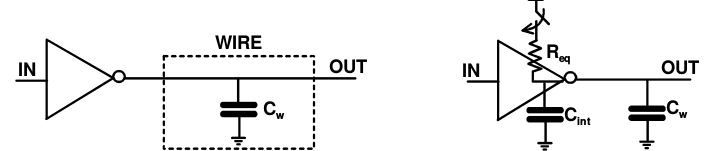
\includegraphics[width=0.5\textwidth]{C5_4.png}\\
\raggedright

The wire capacitance has to be added to the intrinsic capacitance of the inverter in order to correctly estimate the propagation delay that in this case is 
\begin{equation}
\tau=\ln(2)R_{eq}(C_{int}+C_w)
\end{equation}



\subsection{Lumped RC model}
When the resistance is no more negligible a first odrer approximation is to model the wire as it's single equivalent resistace and capacitance 

\centering
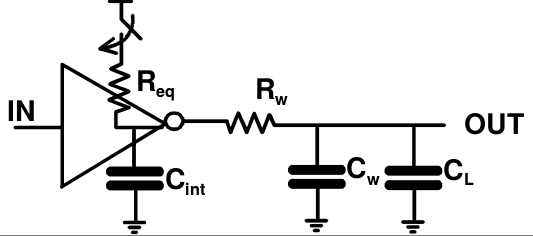
\includegraphics[width=0.35\textwidth]{C5_5.png}\\
\raggedright

To estimate the overall propagation we can model the circuit as follows and use the Elmore theorem

\centering
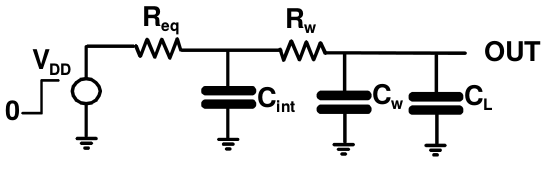
\includegraphics[width=0.35\textwidth]{C5_6.png}\\
\raggedright


\centering

\fbox{\begin{minipage}{40em}
\centering
{\bf Elmore theorem}\\
\raggedright
With a network that has a single input node ,all capacitance between a node and ground and no resistive loops we can assest the propagation delay of the line as calculating for every capacitance C of the network the so called shared-path resistance. This resistance represents the resistance shared between the path from the source of the signal and the output and the path form the source to the capacitance.\\

\centering
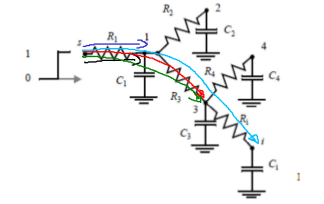
\includegraphics[width=0.35\textwidth]{C5_7.png}\\
\raggedright

\begin{equation}
\tau=C_1R_1+C_2R_1+C_3(R_1+R_3)+C_4(R_1+R_3)+C_j(R_1+R_2+R_j)
\end{equation}

\end{minipage}}

\raggedright
\vspace{5mm}

This is an approximation that brings us to an overestimation of the propagation delay (factor 2) beacuse we are supposing all parasitic terms concentrated in one point and not distributed over a line.\\

\subsection{Distributed model}
With the distributed model we divide the wire into lot of wires of length $\Delta L$ with $\Delta L \rightarrow 0$.\\

\centering
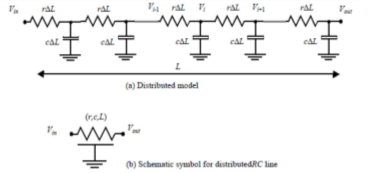
\includegraphics[width=0.5\textwidth]{C5_8.png}\\
\raggedright

In this way through the resoluton of a differential equation for the voltage over the line we get that the delay of the wire is 
\begin{equation}
\tau_w\simeq \ln(2)\frac{R_wC_w}{2}
\end{equation}
That is the correct value wrt the lumped RC model.\\

To correctly take into account the effects of the distribution we will use the following 2 models that give us both the same result of the distributed model

\centering
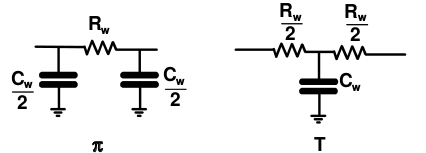
\includegraphics[width=0.35\textwidth]{C5_9.png}\\
\raggedright


\section{Buffering of a line}

If the time constant of a line it's the dominant contribution for delay in our digital circuit it's worth in order to get a faster respnce to cut the wire in N pieces adding buffer in the middle.\\
This is convenient if
\begin{equation}
L\ge\sqrt{\frac{16C_{int}R_{eq}}{cr}}
\end{equation}
where $C_{int},R_{eq}$ are parameters of the driving circuit and c,r are the specific resistance ($\Omega/m$) and capacitance ($F/m$) of the wire.
The optimum number of division N (and so the number of inverter to be added N-1) is
\begin{equation}
N=\sqrt{\frac{R_wC_w}{4C_{int}R_{eq}}}=L\sqrt{\frac{rc}{4C_{int}R_{eq}}}
\end{equation}
And the contribution to $\tau_p$ of the wire ($R_wC_w/2$) decreases by a factor N.\\
The propagation delay of an optimized line that is broken in N peices is 
\begin{equation}
\tau_p=\ln(2) N \left(R_{eq}C_{int}+(R_{eq}+\frac{R_w}{2N})\frac{C_w}{N}+(R_{eq}+\frac{R_w}{N})C_{int}\right)
\end{equation}
In this expression we supposed inverters with the same size and $\gamma=1$.\\
This optimization of the line it's indipendent form the size of the stage present in the circuit.\\

\section{Inductance}

Parasitic inductances can be neglected if the time of flight of the signal is much less than the minimum propagation delay of the circuit. With a line of length L and the maximum propagation delay of $\tau_{max}$ this translates as 
\begin{equation}
t_{flight}=\frac{L}{\frac{c}{\sqrt{\mu \varepsilon}}}\ \  << \ \ \tau_{max}     
\end{equation}
where tipically $\varepsilon=3.9$.\\
\vspace{5mm}
Another condition that makes the inductance negligible is to have
\begin{equation}
L\ \ <<\ \ \frac{1}{r}\sqrt{\frac{l}{c}}
\end{equation}
where r, l and c are the specific resistance inductance and capacitance.\\
        %The wires
%------------------------------------------------------------------------%
\chapter{FC-CMOS gates}

\section{Sizing of single transistor inside a logic gate}
Once the transistor are placed in order to compute the requested logic function the sizing of the single transistor has to follow this simple rule: the equivalent resistance in the worst case state has to be equal to the one of an inverter of the same size of the gate.\\
Transistor in parallel show a resistance half of a single transistor so considering the following NAND gate with a size equal to 1 the p-mos will have an aspect ratio of 3 and the n-mos of 2 (two transistor of size 2 in series are the equivalent of a transistor of size 1).\\

\centering
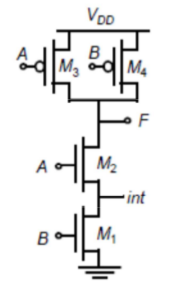
\includegraphics[width=0.15\textwidth]{C6_1.png}\\
\raggedright

If the searched size was s=2 we will have p-mos 6 and n-mos 4 of aspect ratio.\\

\section{Equivalent capacitance}
To estimate the equivalent internal capacitance $C_{int}$ of a generic FC-CMOS gate we have to look to the dimesnions of the transistors connected to the output node. The sum of the aspect ratios of this transistors divided by 4 it's how many $C_g^{(0)}$ the internal capacitance is.\\
\vspace{5mm}
To better assest the propagation delay we should also take into account the inter-nodes capacitance inside our gate; this leads us to a more complex analysis since we have to consider whitch parasitic capacitance are charged an whitch are discharged and we shoulde use the Elmore theorem for every transistion.

\centering
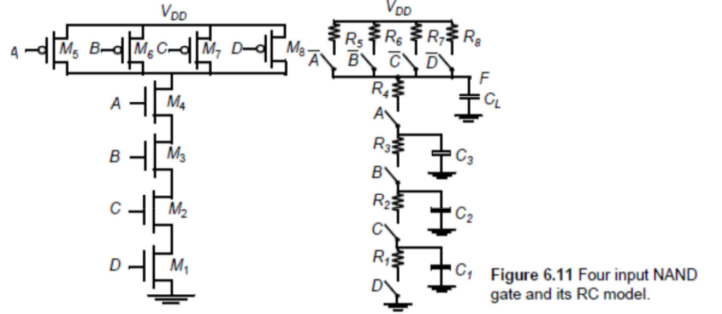
\includegraphics[width=0.5\textwidth]{C6_2.png}\\
\raggedright

This inter-nodes capacitance can't be estimated as before with a value of 2fF but , since 2 transistor in series are integrated with common drain-source, with 1fF capacitance.\\


\centering
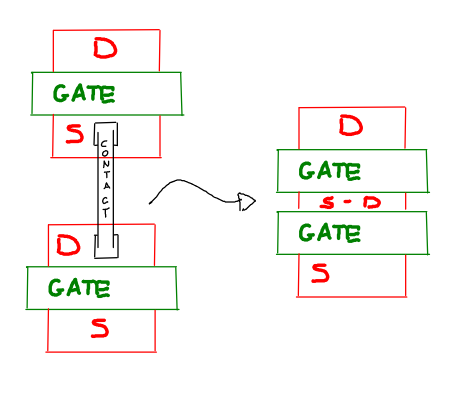
\includegraphics[width=0.35\textwidth]{C6_3.png}\\
\raggedright

We can neglect the effect of the inter-nodes capacitance since our gates have small fan-in (3-4 max).\\

\vspace{5mm}
In case of large fan-in and a lot of transistors in series it's possible to adopt clever sizing "inspired" by the inverter chain optimization 

\centering
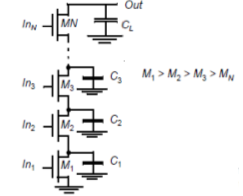
\includegraphics[width=0.35\textwidth]{C6_4.png}\\
\raggedright

\vspace{5mm}
Another good rule of thumb is that the last signal coming to the gate (the slowest signal at the input of the gate) has to be connected to the transistor closest to the output.\\

\section{Propagation delay}

\subsection{Equivalent resistance}
We define the equivalent resistance of a generic gate of size s (built with the right internal proportion described before) as 
\begin{equation}
R_{eq}=\frac{R_{eq}^{(1)}}{s}=\frac{11.6k\Omega}{s}
\end{equation}

\subsection{"p" factor}
The factor "p" or intrinsic delay factor (OUTPUT) it's a constant that connect the intrinsic capacitance of our gate with the intrinsic capacitance of an inverter of the same dimensions and can be calculated as 
\begin{equation}
p=\frac{C_{int}(s=1)}{C_{int}^{(1)}}
\end{equation}
\begin{equation}
p=\frac{\sum \frac{W}{L}|_{mos \ connected \ to \ y}}{4*s}
\end{equation}
and it's releted with the intrinsic capacitance of a generic size gate as 
\begin{equation}
C_{int}=spC_{int}^{(1)}
\end{equation}
This parameter it's indipendent on the size of the gate

\subsection{"g" factor}
The factor "g" is the logical effort (INPUT) that quantifies the complexity of the gate with respect to the inverter in the "input" direction.\\
Also this parameter is indipendent on size and has to be calculated considering single couple of inputs\\ 
\begin{equation}
g=p=\frac{C_{g}(s=1)}{C_{g}^{(1)}}
\end{equation}
\begin{equation}
g=\frac{\sum \frac{W}{L}|_{mos \ connected \ to \ A}}{4*s}
\end{equation}


\vspace{6mm}
\centering
Here some examples of this parameters on famous logic gates\\
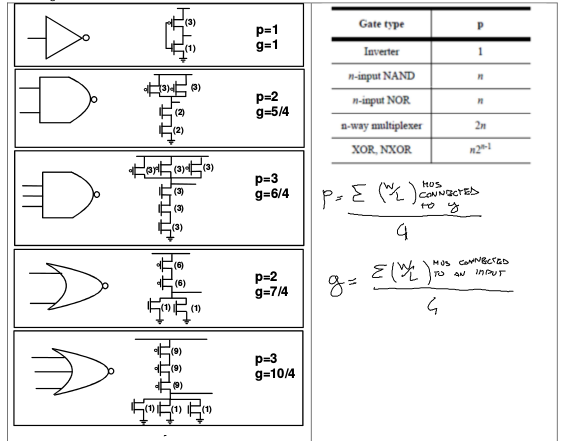
\includegraphics[width=0.75\textwidth]{C6_5.png}\\
\raggedright

\subsection{Propagation delay}
The expression of the propagation delay of a generic gate is
\begin{equation}
\tau_p=\tau_{p0}\left(p+\frac{fg}{\gamma}\right)
\end{equation}
where we can distinguish two contributions; the term $\tau_{p0}$ is the intrinsic delay and $fg\tau_{p0}$  is the effort delay strictly related to the load capacitance. The product fg it's called stage effort or h.\\

\section{Size optimization of $\tau_p$}
The delay that counts and that we are going to optimize it the one related with the critical path, the delay of the longest path.\\
To optimize the propagation delay we need that all the gates have the same stage effort h.\\
\vspace{5mm}
We define the path fan-out as 
\begin{equation}
F=\frac{C_L}{C_{g,1}}
\end{equation}
and the path logical effort as 
\begin{equation}
G=\prod g_i
\end{equation}
To optimize the propagation delay we all the stages has to have the following $h_{opt}$
\begin{equation}
h_{opt}=\sqrt[N]{H}
\end{equation}
This corresponds to a propagation delay of the overall chain of 
\begin{equation}
\tau_{p,opt}=\tau_{p0}\left( (\sum p)+\frac{N h_{opt}}{\gamma} \right)
\end{equation}
in this way the dimension of the j-th stage will be 
\begin{equation}
s_j=\frac{s_1g_1}{g_j}\prod_{i=1}^{j-1}f_i
\end{equation}
or better we can assest every dimension form the first stage to the last one using the formula of $h_{opt}$
\begin{equation}
h_{opt}=f_ig_i \ \ \ \forall i
\end{equation}
using this formula on the i-th stage we will end up with the size of the i+1 stage.

\subsection{Branching}
In the case illustrated in figure we have a so called branching in the path.

\centering
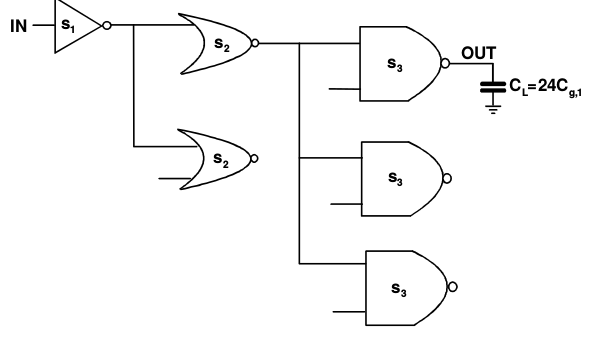
\includegraphics[width=0.35\textwidth]{C6_6.png}\\
\raggedright

There are more stages in parallel (NAND in this case). Under the assumption that all the parallel elements have the same dimensions (all NAND with equal size) we can define the branching factor refering to the extrinsic capacitance as b
\begin{equation}
b=\frac{C_{path}+C_{off-path}}{C_{path}}
\end{equation}
that in practice is the number of stages in parallel (3 in our case).\\
\vspace{5mm}
In this cases we can optimize the chain introducing the path branching factor B
\begin{equation}
B=\prod_{i=1}^N b
\end{equation}
than the way to optimize the chain is the same as before but the H is now defined as 
\begin{equation}
H=FGB
\end{equation}
the number of stages n does not takes into account the braching stages and so to find the size of the single stages we can use the relation
\begin{equation}
h_{opt}=\sqrt[n]{H}=f_ig_ib_i
\end{equation}


\section{Power dissipation}
The consideration on power dissipation are the same for the simple NOT circuits we've done in the previous chapter. The difficult topic here is to assest the parameter $\alpha_{sw}$ and to reason if some states are correleted each other.
\vspace{5mm}
Assuming that the inputs are independent and uniformly distributed, any N-input static gate has a transition probability that corresponds to
\begin{equation}
\alpha_{sw}=\frac{N_0N_1}{2^{2N}}=\frac{N_0(2^N-N_0)}{2^{2N}}
\end{equation}
where $N_0$ and $N_1$ are the number of zero and one, respectively, in the truth table of the logic function.
\vspace{5mm}
Here follows an example where the above formula doesn't work since the 2 inputs are correlated


\centering
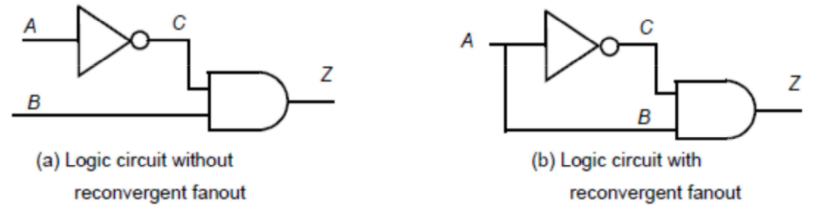
\includegraphics[width=0.7\textwidth]{C6_7.png}\\
\raggedright




















        %FC-CMOS gates
%------------------------------------------------------------------------%
\chapter{Ratioed logic}
Ratiohead logic means that the characteristics of the circuit (statics and dynamics) depends on the ratio between the pull-up and the pull-down network.\\
This type of circuits the advantage of being less area consuming and with small output capacitance.\\

\section{Pseudo-NMOS}
The basic idea behind this logic is to use the same pull down network of an FC-CMOS implementation but using as pull up only a p-mos always on (with the gate grounded)

\centering
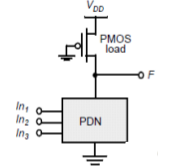
\includegraphics[width=0.35\textwidth]{C7_1.png}\\
\raggedright
       		
Obviously to pull down the output node the pull down network have to be stronger than the p-mos.\\
We drastically reduced the number of transistors form 2N+1 of the FC-CMOS logic to N+1 and doing so also the input and output capacitance.\\

\subsection{Static characteristics}
Let's take as example the pseudo-NMOS inverter

\centering
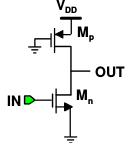
\includegraphics[width=0.2\textwidth]{C7_2.png}\\
\raggedright

$V_{OH}$ remains at VDD but $V_{OL}$ isn't at 0V since both transistors are on when the pull-down network is enabled.\\
Therefore we can estimate that $V_{OL}$ it's close to ground so we can found it's value supposing the pmos in velocity saturation and the nmos in ohmic region and comparing the currents when the input is at VDD and out at $V_{OL}$
\begin{equation}
k'_n \left(\frac{W}{L}\right)_n   V_{OL}(V_{DD}-V_{tn}-\frac{V_{OL}}{2})=k'_n \frac{W}{L}|_p V_{satp}(V_{DD}-V_{tp}-\frac{V_{satp}}{2})
\end{equation}
$V_{OL}$ stricktly depends on the relative ratio between nmos and pmos. Weaker pmos smaller the output voltage low.\\

\vspace{5mm}

Regarding the switching threshold we can suppose it's near the middle and write the ballance of currents with both transistors in velocity saturation where we find the term $V_M$ only in the nmos current
\begin{equation}
k'_n \left(\frac{W}{L}\right)_n  V_{satn}(V_{M}-V_{tn}-\frac{V_{satn}}{2})=k'_n \left(\frac{W}{L}\right)_p V_{satp}(V_{DD}-V_{tp}-\frac{V_{satp}}{2})
\end{equation}
then after getting the first value we can verify if our supposion was right and iterate.\\

\vspace{5mm}

Main drawback of this technology is the static power consumption that we have in correspondance of a logic 0.\\
This power can be evaluated as 
\begin{equation}
P_{static}=P(0)V_{DD}\cdot k'_n \left(\frac{W}{L}\right)_p V_{satp}(V_{DD}-V_{tp}-\frac{V_{satp}}{2})(1+\gamma_p(V_{DD}-V_{OL}))
\end{equation}

\subsection{Dynamic characteristics}

The intrinsic propagation delay can be evaluated in the same way as the FC-CMOS logic restoring the idea of equivalent resistance.\\
In the pull-up time we have to consider that it's an overestimation since we don't start from 0V but from $V_{OL}$.\\
In the pull-down time we're doing an underestimation since the pmos is on and try to charge the capacitance. In order to take into account this effect we can consider the pull-down resistance as
\begin{equation}
R_{pull-down}=\frac{R_{eq,n}}{1-\frac{R_{eq,n}}{R_{eq,p}}}
\end{equation}
Hidden in this relation there is the fact that if the pmos is too strong we aren't able to pull down the y node (for $R_n<R_p$, $R_{pd}$ becomes negative).\\

\vspace{5mm}

There is a trade off between static and dinamic proprieties as the following scheme shows

\centering
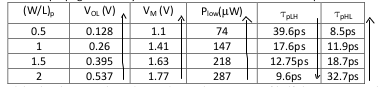
\includegraphics[width=0.5\textwidth]{C7_3.png}\\
\raggedright





\section{DCVSL}
This technology is an improvement of the pseudo-NMOS logic that eliminates the problem of static power consumption and makes the $V_{OL}=0$ using a positive feedback and a differential structure.\\
The basic structure is shown in figure 

\vspace{2mm}
\centering
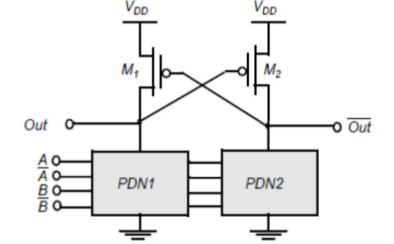
\includegraphics[width=0.35\textwidth]{C7_4.png}\\
\raggedright
\vspace{2mm}

The two pull-down network are complementary and we have a differential output.\\
At steady state there is no conductive path between the voltage supply and ground and the low output voltage is restored due to the feedback loop.\\
Although the logic is still ratioed since if the pull down network is not stronger than the PMOS transistor, the corresponding output node cannot be driven low.\\

\vspace{5mm}

This logics has still some problems since we have cross-conduction current the switching activity is increased ($\alpha_{sw}\simeq 1$) and the cross-connection between the two pmos as the differential naure can be troublesome.\\
















        %Ratioed logic
%------------------------------------------------------------------------%
\chapter{Other static logics}
%------------------------------------------------------------------------%
\section{Pass-transistor}
This technology aim is to reduce the number of transistor with the idea to drive the mos by the gate and olso by the drain/source trerminal. It's a technology suited to implement adders and multipilers.\\
The main idea is to wathc the truth table of our function and think how to implement it as a multiplexer like in figure 

\centering
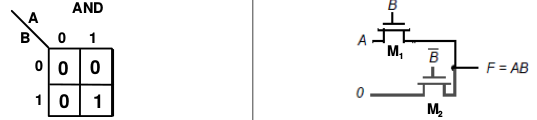
\includegraphics[width=0.35\textwidth]{C8_1.png}\\
\raggedright
 
The signal B is used as a selector.\\
This type of implementation has a lot of drawback since the nmos transistors are not good at charging capacitance they are affected by body effect so on the output node we have $V_{DD}-V_{tn}*$ that creates crossconduction current if it's connected to an inverter and it's the reason why it's forbidden to cascade pass-transistor.\\
%------------------------------------------------------------------------%
\subsection{Pass-transistor with level restorer}

First try to fix this issues is to use a level restorer in order to restore the voltage only to ground or power supply without consuming static power consumption using a classical inverter and a pmos 

\centering
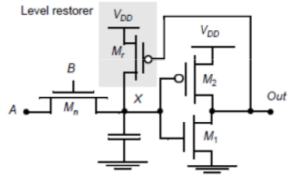
\includegraphics[width=0.35\textwidth]{C8_2.png}\\
\raggedright

The logic is still ratioed since the ratio of dimensions between the pass-transistor and the pmos it's foundamental since the pass-transistor have to be able to drive the X node low.\\
%------------------------------------------------------------------------%
\subsection{Swing restored pass transistor logic}

If we want a differential implementation of the pass-transistor logic we can employ two inverters in a crosscoupled fashon instead of the voltage restores and two complementary pass-transistor network.\\

\centering
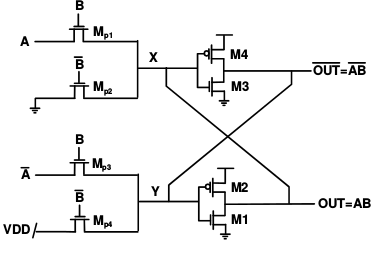
\includegraphics[width=0.35\textwidth]{C8_3.png}\\
\raggedright

The problem is again that this is still a ratioed implementation and a right sizing is mandatory to let this circuit work fine.\\




%------------------------------------------------------------------------%
%------------------------------------------------------------------------%
\section{Complementary pass-transistor logic CPL}
The final solution to the problems of the pass-transistor logic is the complementary pass transistor logic where we have two level restorers with gate connected to the opposite pass-transistor block and and two inverters that operates as buffer to permit the cascade of other logic ports.\\

\vspace{5mm}
\centering
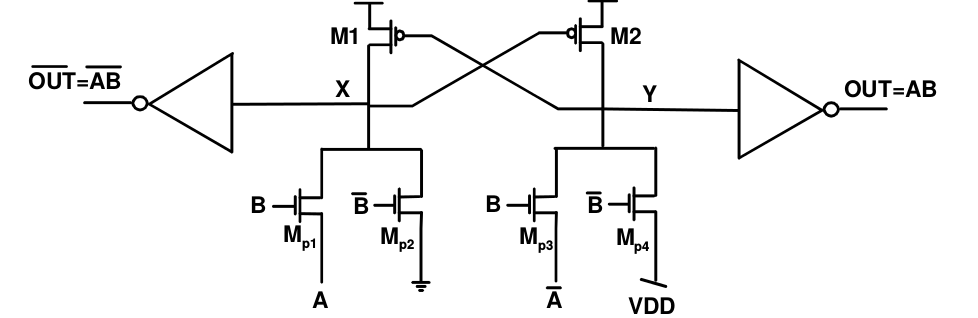
\includegraphics[width=0.5\textwidth]{C8_4.png}\\
\raggedright
\vspace{5mm}

This logic is ratioless since the feedback loop heps the transition and the on-off state of the two pmos transistors.\\
\vspace{5mm}
To build the pull down networks we have 2 different method: mux way or intuituve way.\\
In the multiplexer way we decide witch signals activate the mos and the signal that will be used as output than we can do some semplification limiting ourself to a tree structure like in figure

\vspace{5mm}
\centering
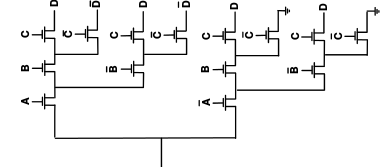
\includegraphics[width=0.5\textwidth]{C8_5.png}\\
\raggedright
\vspace{5mm}

The second way is to find on the k-map some groups of bits that corresponds to some condition like in figure

\vspace{5mm}
\centering
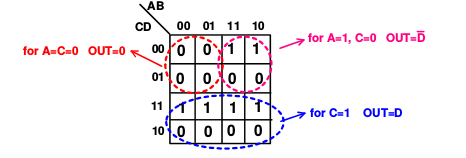
\includegraphics[width=0.5\textwidth]{C8_6.png}\\
\raggedright
\vspace{5mm}

\subsection{Propagation delay}
{\bf Low to high $\tau_{lh}$}\\
A low to high transition on the output Y corresponds to a high to low transition before the inverter so the nmos are discharging the intrinsic capacitance $C_{int}$.\\
The time taken by the system to discharge this capacitance is 
\begin{equation}
\tau'=\ln(2)R_nC_{int}
\end{equation}
where $R_n=13k$ as usual.\\
So the oveall time for a low to high transition is $\tau'$ plus the low to high propagation delay of the inverter that is 12ps
\begin{equation}
\tau_{lh}=\ln(2)R_nC_{int}+\tau_{plh}^{inv}=\ln(2)13kC_{int}+12ps
\end{equation}

\vspace{7mm}
{\bf High to low $\tau_{hl}$}\\
A high to low transition on the output Y corresponds to a low to high transition before the inverter so the nmos are charging the intrinsic capacitance $C_{int}$.\\
Thus we can't use the usual value of the resistance but we have to calculate the value considering an initial with source at 0V an final condition of the mos with source at $V_{DD}/2$.\\
\vspace{3mm}
\centering
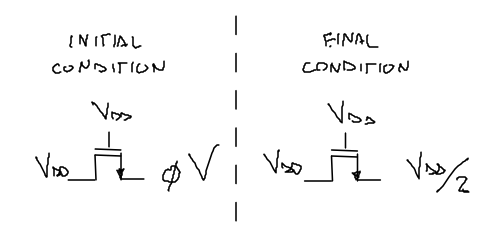
\includegraphics[width=0.55\textwidth]{C8_01.png}\\
\raggedright

Considering the body effect in the initial condition we are in velocity saturation but at the end in pinch off saturatio ($V_{tn}^{*}\simeq0.7-0.8$) so we can compute the equivalent resistance as 
\begin{equation}
R_{eq,n}=\frac{1}{2}\left(\frac{V_{DD}}{I_{vsat}^{(i)}}+\frac{V_{DD}/2}{I_{po}^{(f)}}\right)
\end{equation}
that depends on the equivalent reistance dimensions and it's the dominant term in the overall delay.\\
The high to low equivalent delay will be 
\begin{equation}
\tau_{hl}=\ln(2)R_{eq,n}C_{int}+\tau_{phl}^{inv}=\ln(2)R_{eq,n}C_{int}+18ps
\end{equation}

%------------------------------------------------------------------------%
\section{Trasmission gate}
Another solution to avoid the voltage drop problem is the use of trasmission gates that are one nmos and one pmos in parallel that are driven by complementary signals.\\
This device acts as a switch since turns on or off both devices. The advantage is that in this way we can always discharge/charge totally the load without stopping at a threshold voltage of distance.\\

\centering
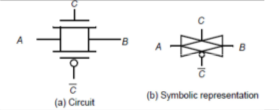
\includegraphics[width=0.35\textwidth]{C8_7.png}\\
\raggedright






























































        %Other static logics
%------------------------------------------------------------------------%
\chapter{Dynamic logic}
Until now we have studied static logics in whitch the output node it's always connected to gnd or $V_{DD}$ through a low impedance path.\\
Dynamic logics feature high impedance at the output and the information is stored in a capacitance.\\


\section{Static and dynamic proprieties}

This technology reduce the capacitances (both input and output) by using a single clocked pmos transistor (and a clocked nmos too)

\centering
\includegraphics[width=0.35\textwidth]{C9_1.png}\\
\raggedright

This device has 2 phases: pre-charge and evaluation.\\
When CLK=0 we are in the pre-charge phase the pull-down network is disabled by the last nmos and the clocked pmos charge the output capacitance.\\
When CLK=1 we are in the evaluation phase the pull-down network is enabled and if the inputs are high than the output capacitance can be discharged. In order to the gate to work proprely during this phase the input signals can have only low to high transitions or they can remain stable (if they have a h-l commutation the output cannot change to high).\\
\vspace{5mm}
The logic function is implemented by the pull-down network that is the same of an FC-CMOS gate. The overall number of transistor is reduced at N+2 without losing the ratioless propriety. Reducing the number of transistors also the capacitance are reduced therefor we get an increase of speed.\\
\vspace{5mm}
Noise margins cannot be evaluated since we can't draw a characteristics but we can say that NMH$\simeq V_{DD}-V_{tp}$ and NML$\simeq V_{tn}$.\\
\vspace{5mm}
The positive aspects of this technology is that both input and output capacitance are smaller and we avoid any short circuit current with ideal clock signal.\\
However we have consider that we have another source of power dissipation that is the clock and that the switching activity is larger since p(1)=1 so 
\begin{equation}
\alpha_{sw}=p(0)
\end{equation}

\section{Issues in dynamic logic}
There are several issues that have to be take into account to verify that the circuit works proprely


\subsection{Leakage current}

\vspace{3mm}
\centering
\includegraphics[width=0.5\textwidth]{C9_2.png}\\
\raggedright
\vspace{3mm}

If the clock frequency is very low sketching the output voltage, we can observe that it does not remain at $V_{DD}$ during the evaluation phase but slightly decreases. This effect is due to the leakage current.
This is a problem only at low frequency of the clock when the voltage across the capacitance can decrease more than $V_{DD}/2$.\\
\vspace{5mm}

We can use two solutions to avoid this drawback.\\
\tab I) Adopt a bleeder that keeps the output node at high level during the evaluation phase. But in this way we restore the ratioed problems so the transistor has to be correctly sized in order to be let the pull-down network dominate.\\
\tab II) Use a pmos transistor in feedback configuration that operates only if the output voltage is high. This is still a ratioed solution since if the output is high and the pull-down network is enabled the pmos has to be enought weak to let the nmos prevail and discharge the capacitance

\centering
\includegraphics[width=0.45\textwidth]{C9_3.png}\\
\raggedright


\subsection{Charge sharing}
This is a problem of the inter-nodes parasitic capacitances that until now we've negleced.\\
Let's consider a 2 input NAND

\centering
\includegraphics[width=0.25\textwidth]{C9_4.png}\\
\raggedright

If we are in the pre-charge phase and the input A toggles we have a charge sharing problem that varies the output voltage.\\
We can separate two cases large variation of the output or small variations.\\
\vspace{3mm}
For large variation of the output voltage ($\Delta V_{out}=V_{DD}-V_{out}\ge V_{tn} $) at the end the source of Ma will be the same as the output voltage at the end so we get that 
\begin{equation}
\Delta V_{out}=V_{DD}\frac{C_A}{C_L+C_A}
\end{equation}

\vspace{3mm}
For variations smaller than the nmos threshold the voltage at the source grows but cannot reach the output since the mos is shut off earlier.\\
In this case 
\begin{equation}
\Delta V_{out}=(V_{DD}-V_{tn})\frac{C_A}{C_L}
\end{equation}

\vspace{3mm}
The case change with the value of the ratio of the two capacitance; equating  the two equation to $V_{tn}$ we get that the limit is (considering also the body effect
\begin{equation}
\frac{C_A}{C_L}=\frac{V_{tn}}{V_{DD}-V_{tn}} = 0.38
\end{equation}
This means that $C_A$ has to be smaller than 0.38$C_L$.\\


\vspace{5mm}
The solution is to precharge also the internal node as in figure

\centering
\includegraphics[width=0.15\textwidth]{C9_5.png}\\
\raggedright

\subsection{Capacitive coupling}

\centering
\includegraphics[width=0.35\textwidth]{C9_6.png}\\
\raggedright

High impedance node are very sensitive to interference and crosstalk so we have to be carefoul in the design of the overall circuit to do not put wires near the output of a dynamic gate in order to avoid interference and "parasitic" toggles due to a switch of the line.
The resulting voltage drop at the output is 
\begin{equation}
\Delta V_{out}=\frac{C_p}{C_L+C_p}V_{DD}
\end{equation}

\subsection{Clock feedthrough}
It's a particular type of clock feedthrough that can cause latch-up problems.\\


\section{Cascading dynamic gates}
The problem in cascading dynamic gates is that only a low to high transition is permitted during the evaluation phase (or a stable signal).\\
We can cascade dynamic gates in two different ways.

\subsection{Domino Logic}

\centering
\includegraphics[width=0.35\textwidth]{C9_7.png}\\
\raggedright

During the pre-charge phase, the output of the dynamic logic is charged up to $V_{DD}$ while the inverter output is driven low. During the evaluation phase, the dynamic gate eventually discharges its output node and the output of the inverter transitions from 0 to 1. Otherwise, it remains low. This ensures that only transitions from 0 to 1 can happen in the evaluation phase.
In this way sequential logic gates are driven by low impendance device increasing the reliability.\\
The main drawback is that it's impossible to implement inverting functions in this way.\\
\vspace{5mm}
Alternative way is to use the unfooted logic (wihout the clocked nmos) or the Dual Rail Domino logic.\\

\centering
\includegraphics[width=0.35\textwidth]{C9_8.png}\\
\raggedright

\centering
\includegraphics[width=0.35\textwidth]{C9_9.png}\\
\raggedright



\subsection{NP-CMOS dynamic}

\centering
\includegraphics[width=0.35\textwidth]{C9_10.png}\\
\raggedright

The idea is to cascade n-type dynamics gate to p-type in order to have always the correct commutation during the evaluation phase (note that both type have simultaniously evaluation and precharge phase).\\




























































































































































        %Dynamic logic
%------------------------------------------------------------------------%
\chapter{Scheme of all the logic families}
\includepdf[pages=1]{Logic_families_scheme_v1.pdf}
    %Scheme of all logic families
%------------------------------------------------------------------------%
\chapter{Sequential circuits}
Sequential logic circuits are such that the outputs depends not only on the present value of the input but also on theyr previous values.
To achive this goal we need gates that have to remember the history of the input data; such circuits are said to have a state.\\
There are 2 basic memory elements: latches and flip-flops.\\
	
\vspace{5mm}

Latches are tipically used to build flip-flops in the master-slave configuration (that is the most adopted memory element). Both latches and flip-flop are in theyr basic configuration a 3 port devices with 2 inputs an 1 output: the two inputs are D data in and CLK clock , the output is Q (and an eventual $\bar{Q}$).\\
\vspace{5mm}
\centering
\includegraphics[width=0.5\textwidth]{C10_1.png}\\
\raggedright
\vspace{7mm}

A latch is a memory element sensitive to the level of the clock, while the flip-flop is sensitive to the edge of the clock signal. We will refer to a latch as to an element level-triggered, and to the flip-flop as an element edge triggered.\\

\vspace{5mm}
\centering
\includegraphics[width=0.7\textwidth]{C10_2.png}\\
\raggedright

\centering
\includegraphics[width=0.7\textwidth]{C10_3.png}\\
\raggedright
\vspace{5mm}

To build up a flip-flop we can use the master-slave structure using 2 latches one positive and one negative connected as shown in figure

\vspace{5mm}
\centering
\includegraphics[width=0.8\textwidth]{C10_4.png}\\
\raggedright
\vspace{5mm}

The main applications for this structrures are four: data sotrage in foreground memory (RAM is a background element), frequency divider, counters and finite state machines (FSM)





\section{Finite state machines (FSM)}

\centering
\includegraphics[width=0.5\textwidth]{C10_5.png}\\
\raggedright

It’s a compound of a logic circuit and one or more flip-flops adopted as memory elements to store data.\\
\vspace{3mm}
There are some importants times that has to be considered when we deal with memory elements
\begin{itemize}

\item The set-up time $t_{su}$ is the time that the input data must be valid before the sensitive edge of the clock.

\item The hold time $t_{hold}$ is the time that the input data must remain stable after the edge of the clock (it can be also negative).

\item If the previous times are verified the input data is copied at the output after a time $t_{cq}$ that is form the edge of the clock to the cross of half supply at the output.

\end{itemize}

For a generic FSM we can underline two time constraints that have to be respected for the circuit to work.\\

\centering
\includegraphics[width=0.5\textwidth]{C10_6.png}\\
\raggedright

\subsection{Max-delay constraint}
Denoting T as the clock period and $t_{p,logic}^{max}$ as the maximum delay of the logic, we have to ensure that 
\begin{equation}
t_{cq}+t_{su}+ t_{p,logic}^{max} \le T
\end{equation}
That can be translated in 
\begin{equation}
t_{p,logic}^{max}\le T-(t_{cq}+t_{su})=T-t_{overhead}
\end{equation}
The signal has to pass throught the flip-flop and the logic and be present at the input od the memory element a set-up time before the edge of the clock.\\

\subsection{Min-delay constraint}
The hold constraint says that the signal cannot propagate throught the flip-flop and the logic too fast or it will remain at the input of the flip-flop for too little time
\begin{equation}
t_{cq}+ t_{p,logic}^{min} \ge t_{hold}
\end{equation}


\section{Static memory devices}

Typical static memory device is a couple of inverter connected in positive loop one another. This type of structure gives us (overlapping the 2 characteristics) has only 2 stable ponis (ground or $V_{DD}$) and one metastable point as shown in figure

\centering
\includegraphics[width=0.7\textwidth]{C10_7.png}\\
\raggedright

\subsection{Multiplexer-based static latch}

\centering
\includegraphics[width=0.5\textwidth]{C10_8.png}\\
\raggedright

The loop can be opened to write the data or closed to store it. The mux is implemented with transimssion gates as in figure (positive latch in figure)

\centering
\includegraphics[width=0.35\textwidth]{C10_9.png}\\
\raggedright

Since when implementing a clocked element the number of transistors connected to the clock signal play a foundamental role in power dissipation (since theyr $\alpha_{sw}=1$) we can also use this structure

\centering
\includegraphics[width=0.35\textwidth]{C10_10.png}\\
\raggedright

This structure has of course some drawbacks; the nmos passes a degraded high voltage that implies a larger propagation delay, reduced noise margins and static power consumptions of the inverters.\\


\subsection{Multiplexer-based static flip-flop}

The multiplexer-based static flip-flop is implemented in the master-slave configuration as follows

\centering
\includegraphics[width=0.7\textwidth]{C10_11.png}\\
\raggedright

We define $t_{inv}$ as the propagation delay of the inverter and $t_{tx}$ as the propagation delay of a trasmission gate; doing so we can hilight the different time constraint of this device.\\

\begin{itemize}

\item 
{\bf Set-up time}\\
We need that the input signal passes throught the first inverter $I_1$ the trasmission gate $T_1$ and the other 2 inverters $I_2,I_3$ otherwise there is the possibility to have conflicts or incorrect values on the 2,3 inverters so
\begin{equation}
t_{su}=3t_{inv}+t_{tx}
\end{equation}

\item 
{\bf Propagation delay}\\
Due to set-up time we already have the signal after the $I_4$ inverter. The signal have to be propagated throught the trasmission gate $I_4$ and the inverter $I_6$
\begin{equation}
t_{cq}=t_{inv}+t_{tx}
\end{equation}

\item
{\bf Hold time}\\
The rising edge of the clock turns the transmission gate $T_1$ off, thus any change of the input signal does not cause a change of the flip-flop state.
Since the inverter $I_1$ has a propagation delay, the input D can change also before the rising edge of the clock without being sampled by the transmission gate; the hold time is negative
\begin{equation}
t_{hold}=-t_{inv}
\end{equation}

\end{itemize}


\subsection{Time constraints rigorous definitions}

%TO DO%




\subsection{Brute force filp-flop}

To reduce the number of transistors involved in a flip-flop (and also the problem of high number of transistor feeded by the clock signal) we can use a ratioed solution like the brute-force flip-flop

\centering
\includegraphics[width=0.7\textwidth]{C10_12.png}\\
\raggedright

The first latch can be written only if the first trasmission gate and the driver circuit are stroger than the feedback inverter to change the state at the input of $I_1$.\\
Moreover there is a problem of "reverse conduction". When the clock is high the second trasmission gate is closed and there can be a conflict between the first and the second stage; $I_4$ has to be sized in a way that can't overwhelm $I_1$ (if this happen the first loop can change it's state).\\

\subsection{Clock overlap}

Due to different paths the clk and the $\bar{clk}$ signals aren't sincronized but they have a period of overlap (0-0 or 1-1 overalap) that can cause wrong toggles (due to critical races that is that the output is connected to the input in 1-1 overlap) or undefined states (due to 0-0 overlap).\\
\vspace{5mm}
A solution to solve the 1-1 overlap is the adoption of the following circuit to generate the 2 clock signals

\centering
\includegraphics[width=0.5\textwidth]{C10_13.png}\\
\raggedright

\centering
\includegraphics[width=0.5\textwidth]{C10_14.png}\\
\raggedright

There is never a period when both signals are high but on the other hand there are a lot of 0-0 overlaps that can destroy the state if this condition last for too long.\\

\section{Dynamic memory devices}
This memory elements store the data as chage across a capacitance as the dynamics gates. The main drawback is that charge may be lost if the data is not refreshed for a long time.\\
The classical master-slave implementation of a flip-flop reduces to 8 transistors as shown in figure (the capacitance are the parasitic of the trasmission gate and of the inverter)

\vspace{2mm}
\centering
\includegraphics[width=0.7\textwidth]{C10_15.png}\\
\raggedright
\vspace{2mm}

The sensitive times related to this implementation are
\begin{itemize}
\item 
{\bf Set-up time}\\
The time needed to the trasmission gate to pass the data to the node "1"
\begin{equation}
t_{su}=t_{tx}
\end{equation}

\item 
{\bf Propagation delay}\\
Is the time that the data use to pass form the node "1" to the output (the transition throught the inverter has not yet passed)
\begin{equation}
t_{cq}=t_{inv}+2t_{tx}
\end{equation}

\item
{\bf Hold time}\\
The hold time is 0

\end{itemize}
\vspace{5mm}
During both clock overlaps in this gate we get a direct connection between in and out.\\
The 0-0 overlap can be avoided making the overlap period small enough that the signal does not reach the output 
\begin{equation}
t_{overlap-00}\le t_{inv}+2t_{tx}
\end{equation} 
The 1-1 overlap can be avoided establishing a hold time large enough 
\begin{equation}
t_{overlap-11}\le t_{hold}
\end{equation}

\subsection{$C^2 MOS$}
This is a dynamic solution insensitive to clock overlap problems. $C^2$ stand for clocked cmos and the implementation is shown in figure 

\centering
\includegraphics[width=0.5\textwidth]{C10_16.png}\\
\raggedright

The two latches are tristate inverters : the output node can be high low or at high impedance state depending on the inputs. The figure represents a positive edge triggered ff.\\
The only problem that arise is just after a 1-1 overlap as soon as $\bar{clk}$ transit back to 0 the Q node is turned up to $V_{DD}$. This can be solved only imposing a hold time constraint.\\


\subsection{True single phase clock TSPC flip-flops}
This implementation avoid the clock overlap problem by using only the clok signal avoiding it's complement relying on the fact that pmos and nmos are on for different voltages.

\centering
\includegraphics[width=0.5\textwidth]{C10_17.png}\\
\raggedright

When clk is high the circuit is a cascade of two inverters and when the clock is low it's an open circuit in the positive latch and vice versa for the negative so that no direct path can be formed.\\
\vspace{5mm}


To spare transistors we can use the so called "split out" scheme 

\centering
\includegraphics[width=0.5\textwidth]{C10_18.png}\\
\raggedright

The drawback in this case is that the node A cannot feature a full swing leading to worst performance in terms of propagation delay.\\



\section{Scheme of all flip-flops implementations}
\includepdf[pages=1]{ff.pdf}

       %Sequential circuits
%------------------------------------------------------------------------%
%\input{Chapter11}      %Arithmetic logics
%------------------------------------------------------------------------%
%\input{Chapter12}      %Memory cells
%------------------------------------------------------------------------%

\end{document}
